%% ----------------------------------------------------------------
%% Chapter 4 -- Methodology
%% ----------------------------------------------------------------
\chapter{Methodology}
\label{chap:methodology}

In this section, we detail our analytical sensor models, asynchronous state estimation logic and develop the two new fusion algorithms to merge 24~GHz FMCW radar with Wi-Fi FTM.

\section{Sensor Modelling}
\label{sec:sensormodel}

\subsection{Radar Model}
\label{sec:radarmodel}

Our principal spatial sensor is a monostatic 24~GHz FMCW radar operating in the ISM band with a 250~MHz sweep bandwidth. By taking the baseband intermediate frequency (obtained from mixing the transmitted chirp signal with the time-delayed echo), we obtain the target distance via:

\begin{equation}
r = \frac{c \cdot f_{IF}}{2\gamma}
\label{eq:radar_range}
\end{equation}

where $\gamma$ represents the chirp slope. While theoretically, the range resolution of this system would be about 0.6 meters, the on-board firmware uses multi-chirp phase evaluation along with an FFT to generate sub-meter Cartesian coordinates at rates ranging from 10--24~Hz. A microstrip antenna array provides angle of arrival information within a $\pm$60 degree azimuth field of view. All data is collected through UARTs in strict 30 byte frames. A sliding window parser enforces bit-for-bit parity checking for all fields of each frame including frame start, protocol headers, payload lengths, periodic reports commands, coordinate payloads and frame ends. Frames containing errors will be discarded. Once validated Cartesian coordinates have been generated they are immediately transformed into polar form so they can be used as input to the Wi-Fi scalar range model:

\begin{equation}
r = \sqrt{x^2 + y^2}, \qquad \theta = \arctan2(x, y) \times \frac{180}{\pi}
\label{eq:polar_transform}
\end{equation}

All readings below 0.1~m in terms of distance and all readings that exceed the limits of the area we can see are eliminated.

\subsection{Wi-Fi FTM Model and Mitigation of Multipath}
\label{sec:ftmmodel}

In order to eliminate the millimeter wave LOS blockage issue, the system uses IEEE 802.11mc FTM on 2.4~GHz Wi-Fi. An initiator uses round trip times to a cooperative responder for ranging as follows:

\begin{equation}
r_{path} = RTT \times 10^{-12} \times \frac{c}{2}
\label{eq:ftm_basic}
\end{equation}

The physical layer is constrained to HT40 bandwidth, effectively reducing the minimum time resolution by half from 50~ns (spatial resolution of 7.5~m) to 25~ns (spatial resolution of 3.75~m), by forcing tighter preamble correlation peaks. A systematic positive range bias is introduced due to indoor multipath since reflections that are delayed increase the total round trip time. Instead of using arithmetic average, the firmware will request 16 frames per burst of exchanges and then use a minimum RTT heuristic:

\begin{equation}
r_{path} = \min(RTT_{1\dots16}) \times 10^{-12} \times \frac{c}{2}
\label{eq:ftm_min}
\end{equation}

The above minimizes all multipath induced over estimations of the direct path.

\section{State Representation and Kalman Filter Design}
\label{sec:kalman}

Radar transmits data to be used to update locations at rates ranging from 10 to 24~Hz while Wi-Fi sends bursty location measurements at rates ranging from 1 to 2~Hz. Under the common assumption of the standard synchronous Kalman filter model, the rate difference described above creates what we call ``freshness blind'' conditions. During inter-update gaps, the filter trusts stale Wi-Fi readings and tends to pull the estimate toward outdated positions. Upon receipt of another Wi-Fi reading, the filter will then respond in the opposite direction and create the well-known stair-step motion associated with this problem - i.e., track stalls followed by large (non-physical) jumps.

To replace this Zero Order Hold (ZOH) assumption for the prediction step of our Kalman Filter, we have employed a Constant Velocity (CV) prediction model with first order hold (FOH). The number of dimensions of our state space is limited to one dimension (i.e., radial distance) and one dimension (its first derivative), to minimize computation requirements on the embedded microprocessor. Precise inter-measurement timing is obtained via the RTOS kernel function. Radial Wi-Fi velocity is smoothed with an Exponential Moving Average to prevent raw derivative noise from destabilizing the kinematic projection:

\begin{equation}
v_{wifi\_new} = (1 - \alpha)\, v_{wifi\_old} + \alpha \left( \frac{r_{new} - r_{old}}{\Delta t} \right)
\label{eq:ema}
\end{equation}

The smoothing factor alpha equaled 0.3 which results in 70 percent confidence in historical velocity momentum, absorbing high frequency jitter while remaining responsive to sustained acceleration. During communication gaps, the state transition into a predictive coasting phase:

\begin{equation}
r_{pred} = r_{wifi\_last} + v_{wifi\_new}\, \Delta t
\label{eq:coast}
\end{equation}

The formulation ensures that each time a frame is delivered by the fast radar, there will be an equivalent Wi-Fi frame that has been corrected for velocity at that time - eliminating all temporal anomalies in the dual-rate data flow.

\section{Dynamic Covariance Intersection (DCI) Algorithm}
\label{sec:dci}

\subsection{Geometric Projection}
\label{sec:geom_proj}

The radar provides 2-D polar coordinates while the Wi-Fi provides only a single dimension scalar value representing a distance. To convert 1D range information in Cartesian space we need to have an angle which is unavailable accurately when radar is occluded. To resolve this issue, the system has limited fusion to radial components only. Radar is allowed to pass its angular estimate directly and unchanged. This method of performing fusion of the radar and Wi-Fi sensors prevents artificial correlation of angular errors due to past extrapolations from being added to the fusion matrix.

\subsection{Freshness-Weighted Fusion}
\label{sec:freshness}

A standard CI calculates the best convex combination of two estimates that remain consistent with unknown cross correlations among parameters, where the best convex combination is parameterized by $\omega$ between 0 and 1. An innovative aspect of the DCI algorithm is its replacement of static optimization of $\omega$ with a real-time computation of a freshness-based Age of Information penalty. The base variance for both sensors was empirically determined; radar variance was found to be 0.2~m$^2$ reflecting the tight near-field precision; Wi-Fi variance was determined to be 2.0~m$^2$ reflecting the larger multipath variability. The Wi-Fi covariance was modeled as time varying, increasing linearly with process noise over time relative to the last known position measurement:

\begin{equation}
P_{wifi}(t) = \sigma^2_{wifi} + Q \times t
\label{eq:wifi_cov}
\end{equation}

The trust ratio $\omega$ (omega) is calculated during each fusion step based on the instantaneous information ratio:

\begin{equation}
\omega = \frac{1/\sigma^2_{radar}}{1/\sigma^2_{radar} + 1/P_{wifi}(t)}
\label{eq:omega}
\end{equation}

The fused radial estimate can be found as follows:

\begin{equation}
r_{fused} = \left[\frac{1}{\frac{\omega}{\sigma^2_{radar}} + \frac{1-\omega}{P_{wifi}(t)}}\right] \left[\frac{\omega}{\sigma^2_{radar}}\, z_{radar} + \frac{1-\omega}{P_{wifi}(t)}\, r_{pred}\right]
\label{eq:fused}
\end{equation}

During a time when the target is visible, the variance ratio is sufficient to drive radar confidence greater than 91\% and during complete occlusion, the radar covariance increases sharply and the algorithm completely relies on Wi-Fi; therefore, it continues tracking the object even when there are obstructions. This process requires less than 20 operations per step.

\begin{figure}[htbp]
\centering
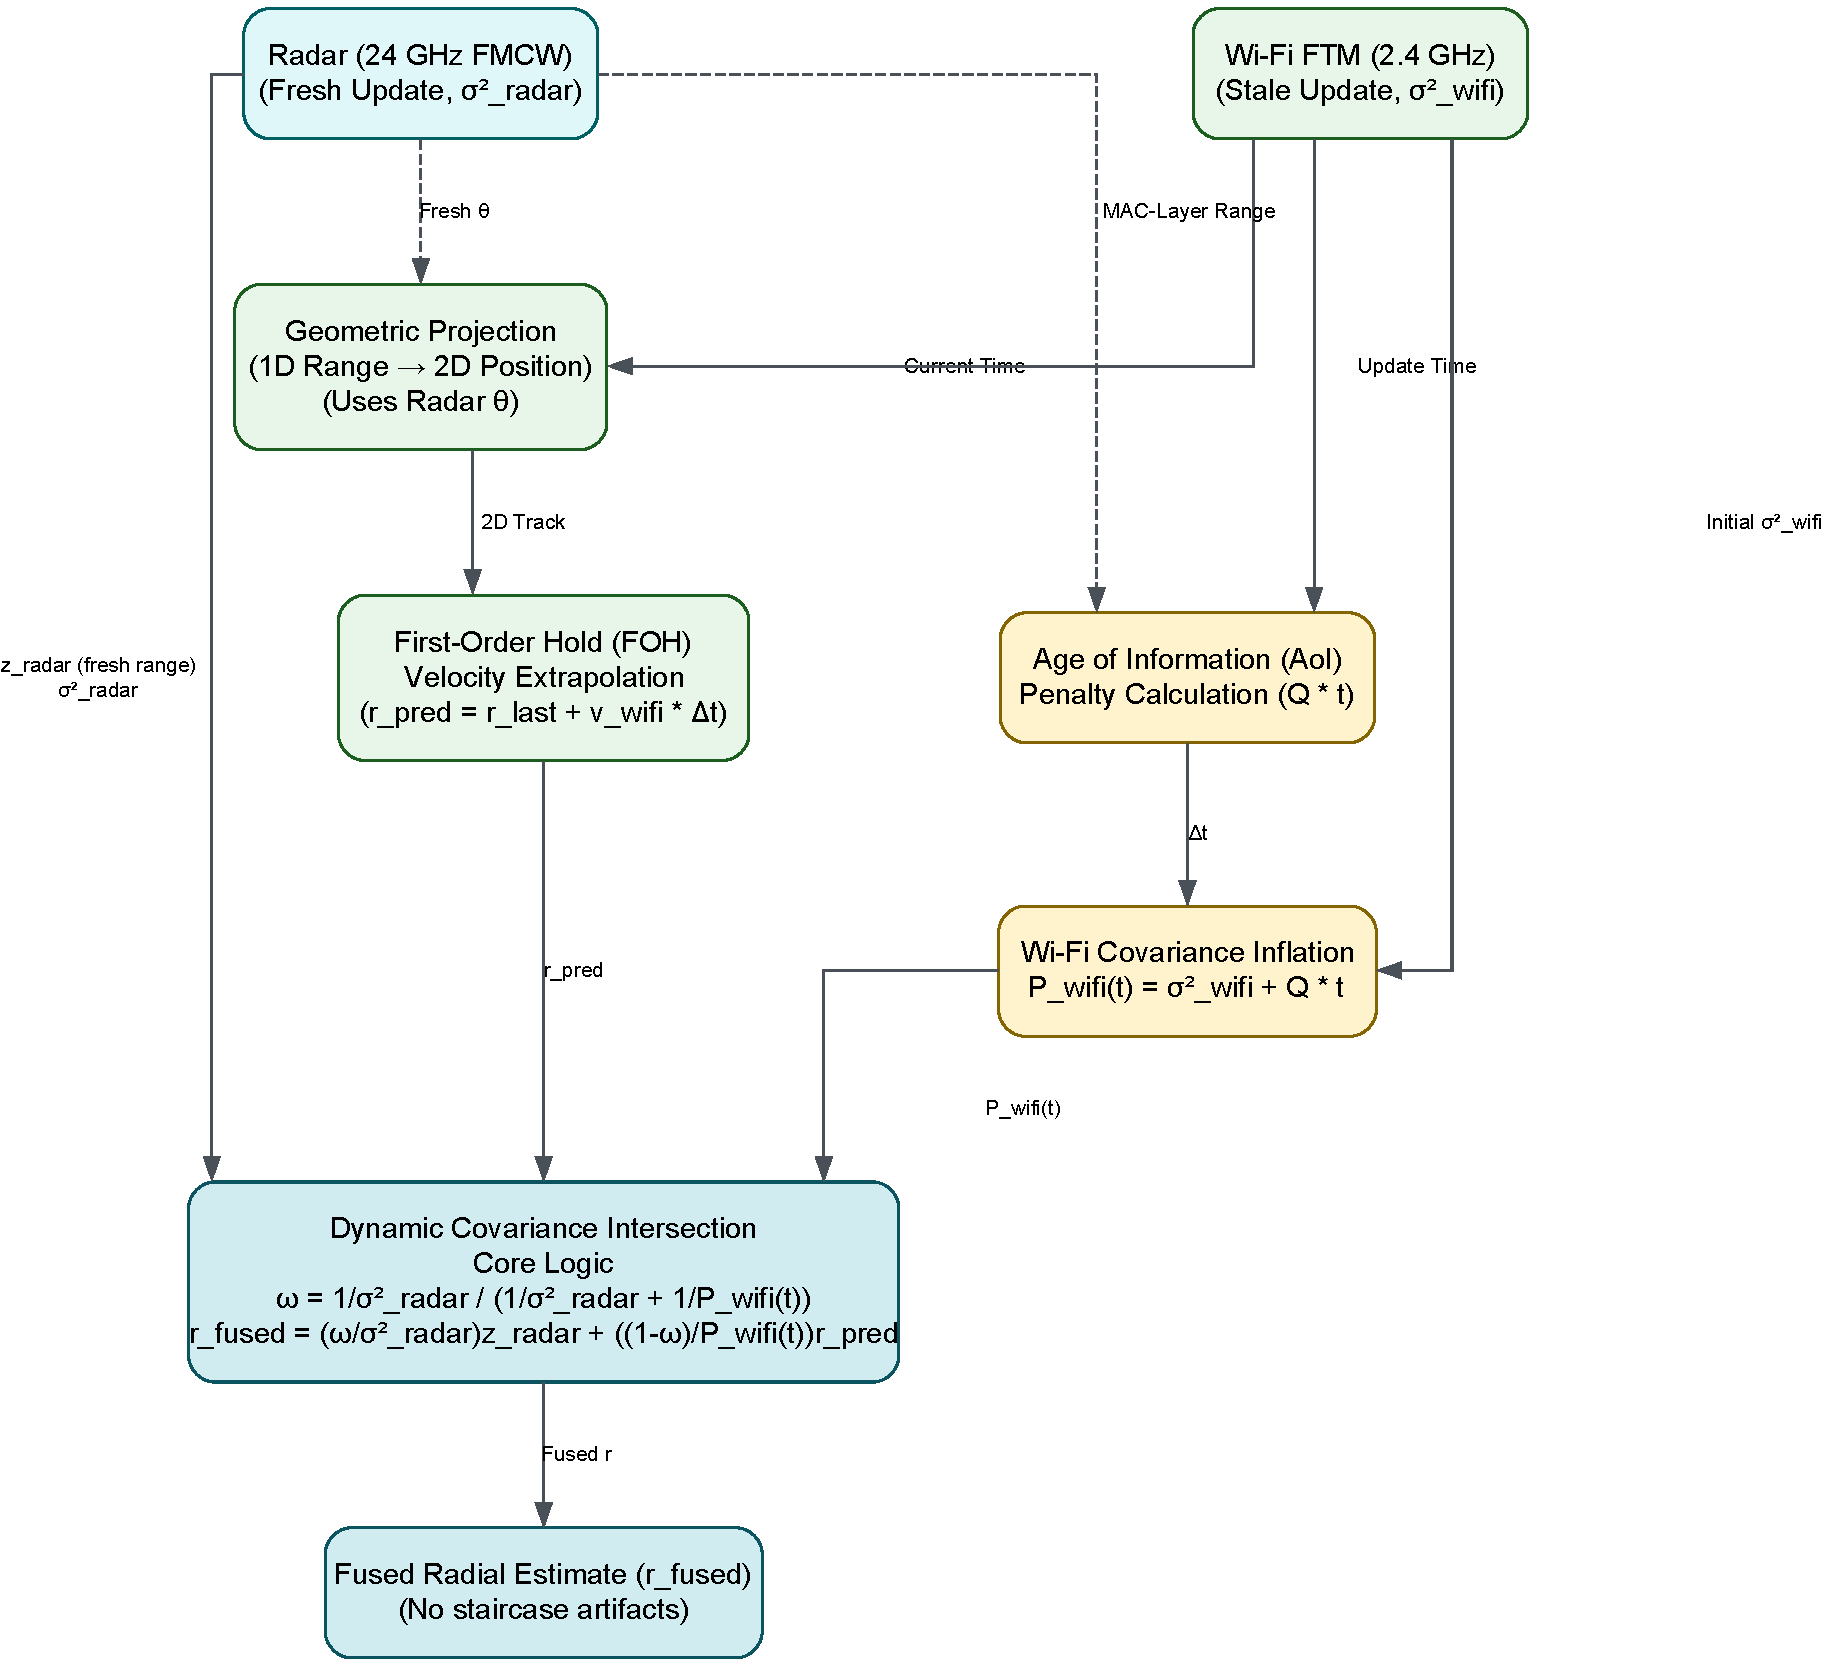
\includegraphics[width=0.8\textwidth]{Figures/DynamicCovarianceIntersectionAlgorithmFlowchart.pdf}
\caption{Flowchart of the Dynamic Covariance Intersection (DCI) algorithm showing freshness-weighted fusion with Age-of-Information penalty.}
\label{fig:dci_flowchart}
\end{figure}

\section{ML-Based Fusion}
\label{sec:mlfusion}

Variance ratios that remain fixed and linear kinematics will not be able to model nonlinear effects of the environment - specifically the inverted error curve, which shows an improvement in Wi-Fi accuracy with increasing distance while the degradation in radar signal also increases with range. An alternative parallel ML-based fusion strategy addresses this limitation.

\subsection{Feature Engineering and Forward-Fill Methodology}
\label{sec:features}

Missing asynchronous readings do not allow the network to recognize a gap in data as being instantaneous movement of the target to the origin; rather, the feature engineering process creates a forward fill method where the last valid reading from the previous step is copied to the current step and a binary freshness flag is added indicating whether or not the value was ``held'' (flag = 0) or if it represented a ``new'' measurement (flag = 1). This enables the network to automatically understand how fast an object moves (decay) through the use of velocity models without explicitly modeling it. In this manner sequential blocks of data are stacked as temporally overlapped sliding windows so that they can be interpreted within kinematic context:

\begin{equation}
X_{train} \in \mathbb{R}^{3488 \times 5 \times 5}
\label{eq:xtrain}
\end{equation}

This includes 3488 samples, a time window of five, and five feature dimensions including; radar distance, radar angle, radar freshness, Wi-Fi distance, and Wi-Fi freshness. All spatial features are clipped at their physical bounds and normalized.

\subsection{Network Structure and Training}
\label{sec:network}

The Multi-Layer Perceptron (MLP) is structured based upon the memory limitations of the microcontroller. The $5 \times 5$ input window was flattened to 25 features, then were two dense hidden layers containing 48 and 24 units respectively, and a final output layer contained two linear units which predict the normalized distance and angle. A total of 2474 units are trainable. Training was accomplished using the Adam Optimizer which minimized mean squared error (MSE) on the data set over 200 epochs with the chronological split of 70\% of the data being dedicated to training, 15\% for validation, and 15\% for testing. The reason for this is to prevent a phenomenon called window-overlap leakage. After seven epochs when there is no change in the loss function, the learning rate is halved and returns to previous best weights if no improvement in validation loss occurs during fifteen consecutive epochs.

\begin{figure}[htbp]
\centering
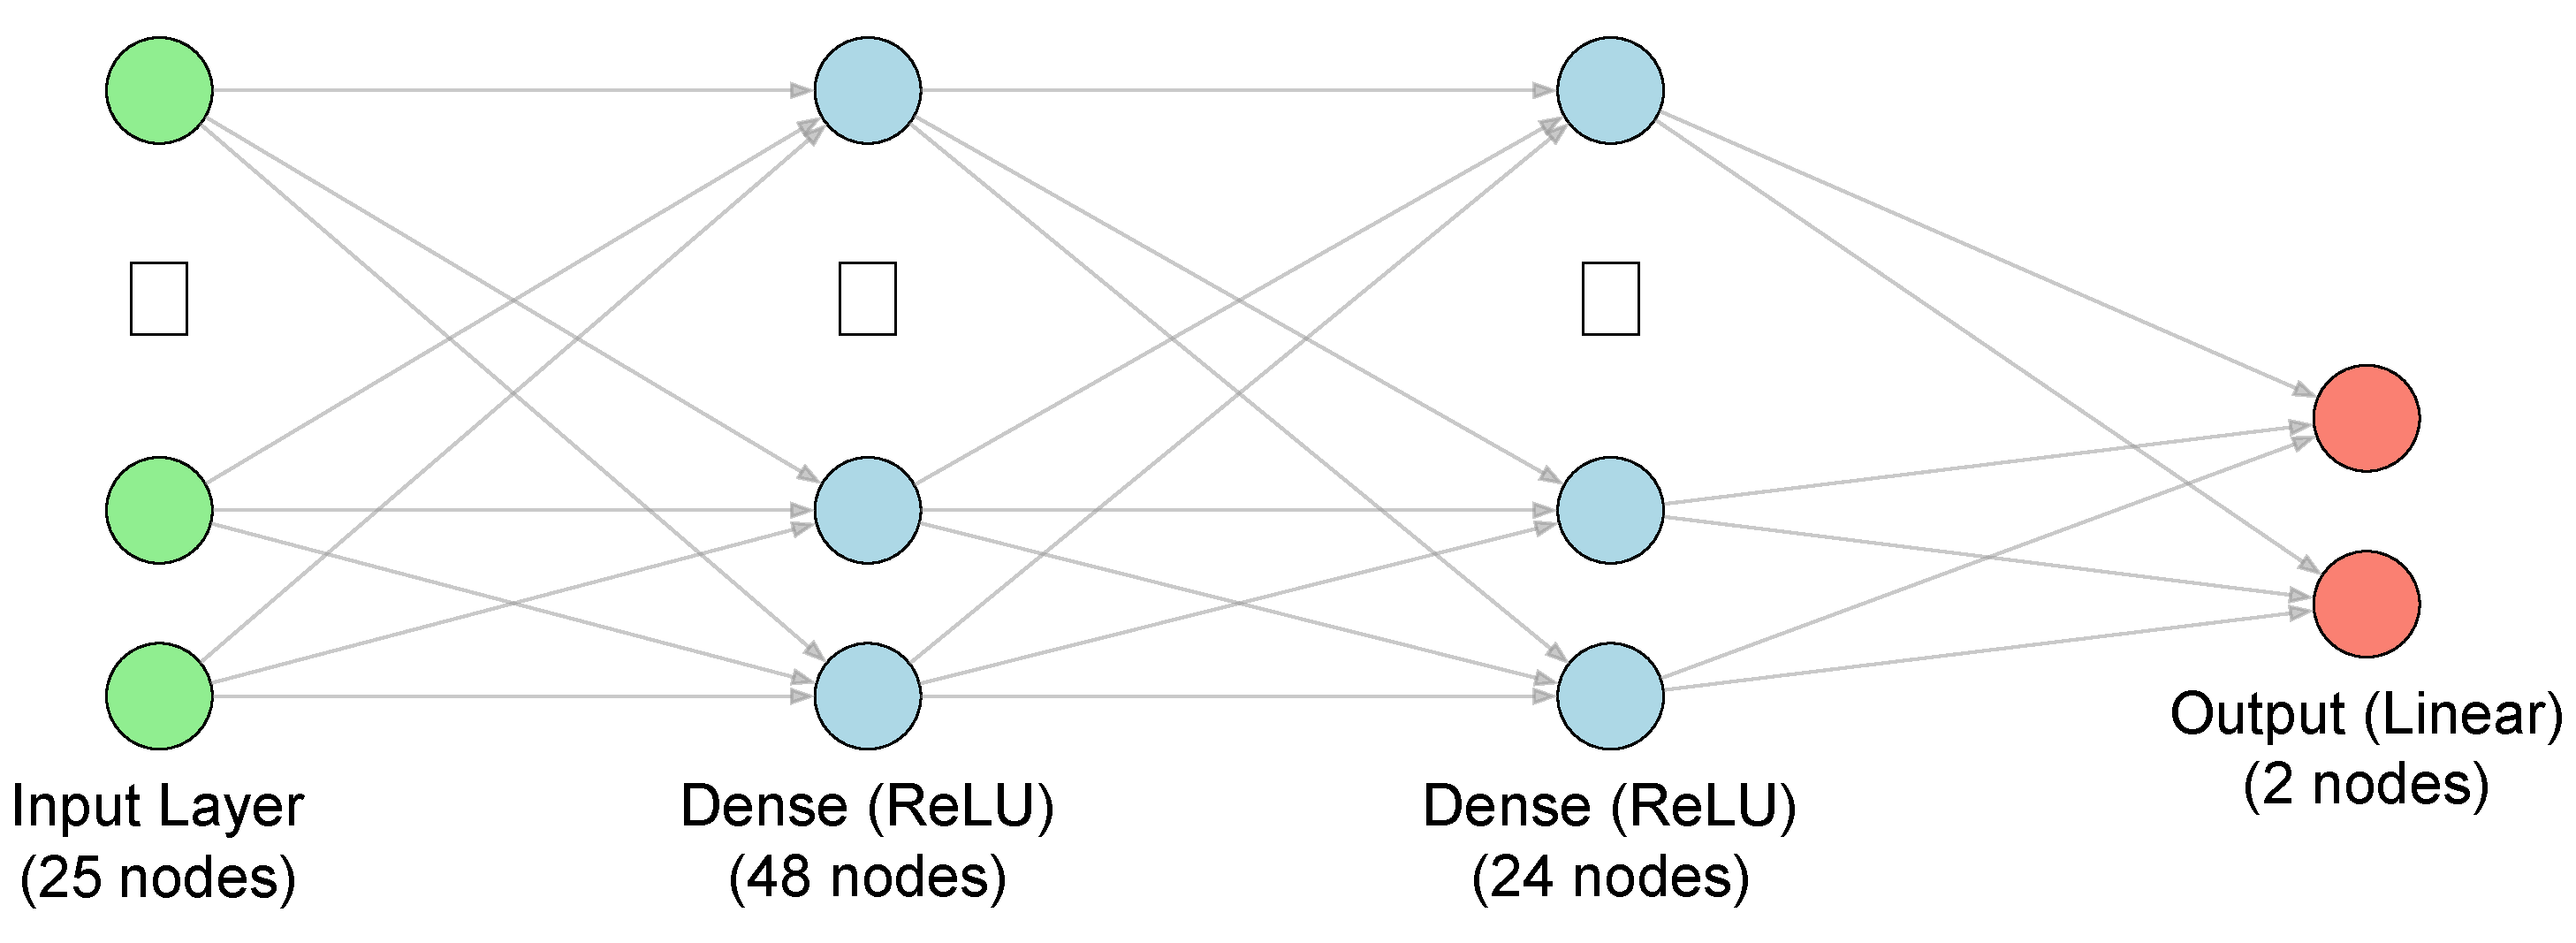
\includegraphics[width=0.85\textwidth]{Figures/MLPmodelNodalDiagram.pdf}
\caption{Nodal diagram of the Edge MLP architecture: 25 input features (flattened $5\times5$ window), two hidden layers (48 and 24 units), and 2 output units (distance and angle).}
\label{fig:mlp_diagram}
\end{figure}

\subsection{Edge Deployment}
\label{sec:edge}

A 2.35~cm geometric floor exists as the result of quantizing a 6~m range into 256 bins which compounding through each layer of hidden processing, with each bin having been defined by a lookup-table approximation for a set of trigonometric functions that may be greatly different than actual value. The unquantized version of this model fits entirely into the 11.6~KB of the internal SRAM (without adding additional latency to access external memory), allowing the model to complete inference in approximately 350 microseconds per window. Execution is strictly isolated to dual-cores. The high speed UART sends bytes quickly; if we were to share a core with the timing interrupt of the Wi-Fi modem's timing interrupt it would fill the serial buffers before they could finish sending them. Wi-Fi operations are executed on Core~0 and all UART parsing/inference will execute on Core~1.

\section{Simulation Environment}
\label{sec:simulation}

Algorithms prior to deployment on embedded systems are tested in two digital twin test environments. In both MATLAB/Simulink environments, continuous time target kinematic models use constant velocity and evasive maneuver generators to simulate motion. In addition to simulating motion, ground truth is degraded via two channels: the Wi-Fi channel samples the data stream at a frequency of 1--2~Hz and adds random Gaussian noise and the radar channel samples at a higher rate but has a configurable signal-to-noise ratio. Interactive parameters can be used to add simulated drops during testing of both the coasting phase and convergence phase.

The track creation module produces line of sight (LOS) trajectories that go through non-LOS scenarios with respect to synthetic barriers. When the radar sensor performs raycasting within its field of vision it also marks an occlusion flag on any obstacle. The WiFi module applies random variance based on distance from the node to simulate actual WiFi signal strength. At 100~ms simulated ticks, the DCI fusion simulates the edge code. In real time users can create virtual walls across trajectories which are immediately detected by the radar and will block the radar's raycasting, causing the radar covariance to spike to infinity. Therefore, all trust is then placed in WiFi. By utilizing this multi-environment paradigm we validate both timing synchronization and geometric covariance behavior prior to testing in a physical environment.

\begin{figure}[htbp]
\centering
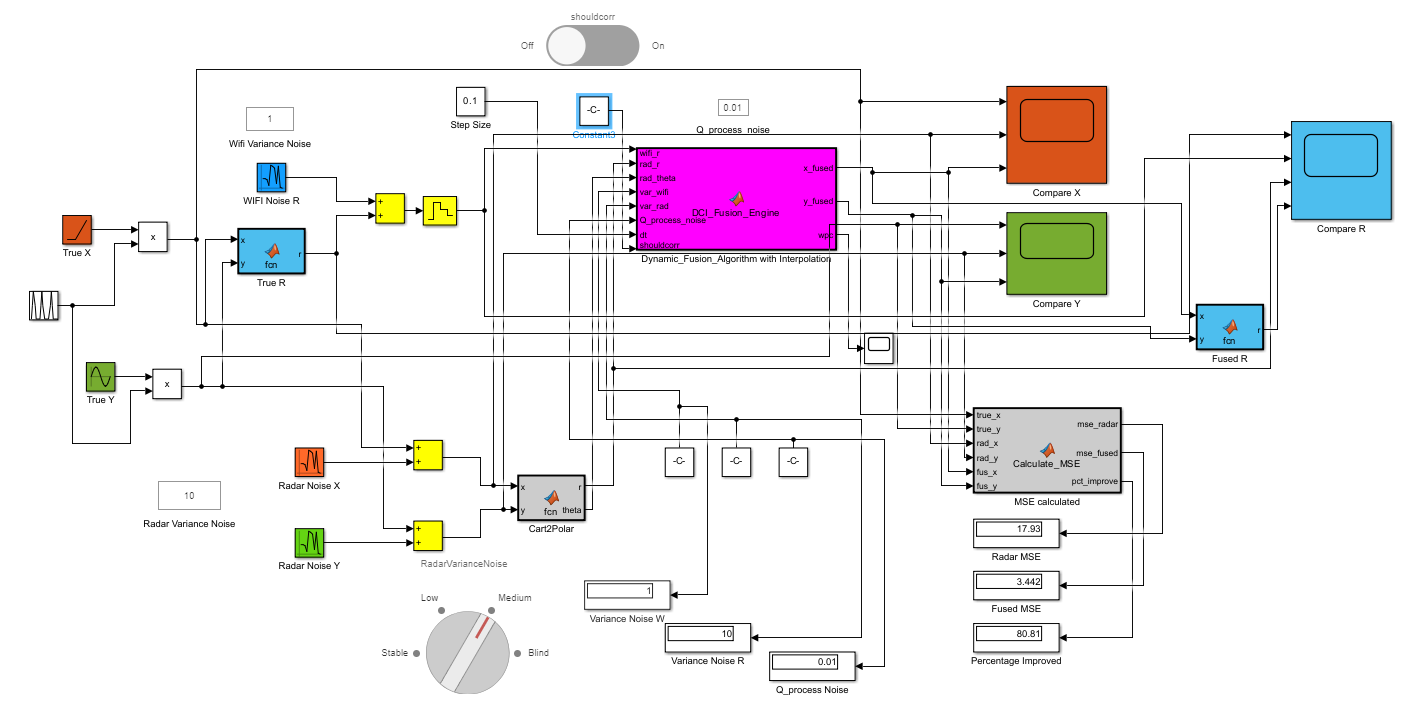
\includegraphics[width=0.9\textwidth]{Figures/DynamicCovarianceAlgorithmMatlabSimulation.png}
\caption{MATLAB/Simulink digital twin simulation of the DCI algorithm showing target trajectory, sensor readings, and fused output with configurable occlusion barriers.}
\label{fig:matlab_sim}
\end{figure}
